% ============================================================
% Relatório EEL891 --- Aprendizado de Máquina --- UFRJ
% Compilar no Overleaf com pdflatex
% Upload: este .tex + ufrj_logo_1.jpeg, ufrj_logo_2.png
%         + eda_preco.png, eda_correlacoes.png, feature_importance.png
% ============================================================
\documentclass[12pt, a4paper]{article}

\usepackage[utf8]{inputenc}
\usepackage[T1]{fontenc}
\usepackage[brazil]{babel}
\usepackage{lmodern}
\usepackage[top=2.5cm, bottom=2.5cm, left=3cm, right=2.5cm, footskip=1.25cm]{geometry}
\usepackage{setspace}
\onehalfspacing
\setlength{\parindent}{1.25cm}
\setlength{\parskip}{0pt}

\usepackage{fancyhdr}
\pagestyle{fancy}
\fancyhf{}
\fancyhead[L]{\small Trabalho 2: Regressão de Preços de Imóveis}
\fancyhead[R]{\small Aprendizado de Máquina (EEL891)}
\fancyfoot[C]{\thepage}
\renewcommand{\headrulewidth}{0.4pt}

\usepackage{graphicx}
\usepackage{float}
\usepackage{caption}
\captionsetup{font=small, labelfont=bf, justification=centering}

\usepackage{booktabs}
\usepackage{tabularx}
\usepackage{array}
\usepackage[table,xcdraw]{xcolor}
\definecolor{headerblue}{RGB}{31,78,121}
\definecolor{rowalt}{RGB}{238,243,248}

\usepackage{listings}
\definecolor{codebg}{RGB}{245,245,245}
\definecolor{codecomment}{RGB}{100,100,100}
\definecolor{codekey}{RGB}{31,78,121}

\lstdefinestyle{pythonstyle}{
  backgroundcolor=\color{codebg},
  basicstyle=\ttfamily\footnotesize,
  keywordstyle=\color{codekey}\bfseries,
  commentstyle=\color{codecomment}\itshape,
  language=Python, frame=single, framerule=0.4pt,
  rulecolor=\color{gray!40}, breaklines=true,
  numbers=left, numberstyle=\tiny\color{gray},
  numbersep=8pt, showstringspaces=false,
  tabsize=2, xleftmargin=1em,
  literate={ã}{{\~{a}}}1 {õ}{{\~{o}}}1 {ç}{{\c{c}}}1
           {á}{{\'a}}1  {é}{{\'e}}1   {í}{{\'i}}1
           {ó}{{\'o}}1  {ú}{{\'u}}1   {â}{{\^a}}1
           {ê}{{\^e}}1  {à}{{\`a}}1
}

\usepackage[colorlinks=true, linkcolor=headerblue, urlcolor=headerblue]{hyperref}
\usepackage{amsmath, amssymb}
\usepackage{enumitem}
\usepackage{titlesec}

\titleformat{\section}{\large\bfseries\color{headerblue}}{\thesection}{1em}{}
\titleformat{\subsection}{\normalsize\bfseries\color{headerblue!80}}{\thesubsection}{1em}{}
\titleformat{\subsubsection}{\normalsize\bfseries\color{headerblue!70}}{\thesubsubsection}{1em}{}

\newcommand{\code}[1]{\texttt{#1}}

\begin{document}
\pagenumbering{gobble}

% ── CAPA ─────────────────────────────────────────────────────
\begin{titlepage}
  \centering
  \begin{minipage}{0.35\textwidth}
    \centering
    
\includegraphics[height=3.2cm]{ufrj_logo_1.jpeg}
  \end{minipage}
  \hfill
  \begin{minipage}{0.58\textwidth}
    \centering
    
\includegraphics[height=3.2cm]{ufrj_logo_2.png}
  \end{minipage}

  \vspace{3.0cm}
  {\LARGE\bfseries EEL891 --- Introdução ao Aprendizado de Máquina\\[0.6em]}
  {\Huge\bfseries\color{headerblue} Trabalho 2 --- Regressão de Preços de Imóveis\\[0.4em]}
  \vspace{0.4cm}
  {\large Estimativa de preço de venda por regressão multivariável}

  \vspace{3.0cm}
  \begin{tabular}{rl}
    \textbf{Aluno:}       & Luiz Felipe Píccoli Cavalini \\[0.5em]
    \textbf{Ferramentas:} & Python 3.12 (\code{scikit-learn}, \code{LightGBM}, \\
                          & \code{XGBoost}, \code{CatBoost}, \code{Optuna}, \code{SciPy}) \\
  \end{tabular}
  \vfill
  {\large Rio de Janeiro, Julho de 2026}
\end{titlepage}

\pagenumbering{roman}
\pagestyle{plain}
\begingroup
  \setlength{\parskip}{0pt}
  \renewcommand{\baselinestretch}{0.95}\normalfont
  \tableofcontents
\endgroup
\newpage
\pagenumbering{arabic}
\pagestyle{fancy}

\section{Introdução}

O presente trabalho consiste na construção de um modelo de regressão multivariável para estimar o preço de venda de imóveis residenciais. A partir de dados históricos de 4.683 imóveis de treino, acompanhados do preço efetivamente praticado, e de 20 características descritivas (tipo, localização, área, quartos, vagas, amenidades, entre outras), o objetivo é predizer o preço de 2.000 novos imóveis cujos preços são desconhecidos.

A métrica de avaliação é o \textbf{RMSPE} (\textit{Root Mean Square Percentage Error}), definida como

\begin{equation}
\text{RMSPE} = \sqrt{\frac{1}{n}\sum_{i=1}^{n}\left(\frac{y_i - \hat{y}_i}{y_i}\right)^2}
\end{equation}

que penaliza o erro \textbf{percentual}, não o erro absoluto: errar R\$~100 mil num imóvel de R\$~200 mil é muito pior do que errar R\$~100 mil num imóvel de R\$~2 milhões. As previsões são submetidas na plataforma Kaggle, que compara automaticamente com o gabarito oculto.

O pipeline adotado segue as etapas clássicas: análise exploratória, pré-processamento (incluindo tratamento cuidadoso de \textit{outliers}), engenharia de \textit{features}, modelagem com múltiplos algoritmos, otimização bayesiana de hiperparâmetros e construção de \textit{ensembles} ponderados. As ferramentas utilizadas foram Python 3.12 com \code{pandas}~\cite{ref:pandas}, \code{scikit-learn}~\cite{ref:sklearn}, \code{LightGBM}~\cite{ref:lgbm}, \code{XGBoost}~\cite{ref:xgb}, \code{CatBoost}~\cite{ref:catboost}, \code{Optuna}~\cite{ref:optuna} e \code{SciPy}~\cite{ref:scipy}.\footnote{O código-fonte completo, incluindo todos os experimentos descritos neste relatório e o histórico de desenvolvimento, está disponível em \url{https://github.com/LuizCavalini/ML-RealEstatePricing}.}

\section{Análise Exploratória dos Dados}

\subsection{Distribuição do preço}

O preço dos imóveis apresenta distribuição fortemente assimétrica à direita, com cauda longa causada por um pequeno número de imóveis de altíssimo valor. Ao aplicar a transformação $\log(1+\text{preço})$, a distribuição se aproxima de uma normal (Figura~\ref{fig:preco}), o que motiva o uso do \textit{target} em escala logarítmica durante o treinamento (Seção~\ref{sec:target}).

\begin{figure}[H]
  \centering
  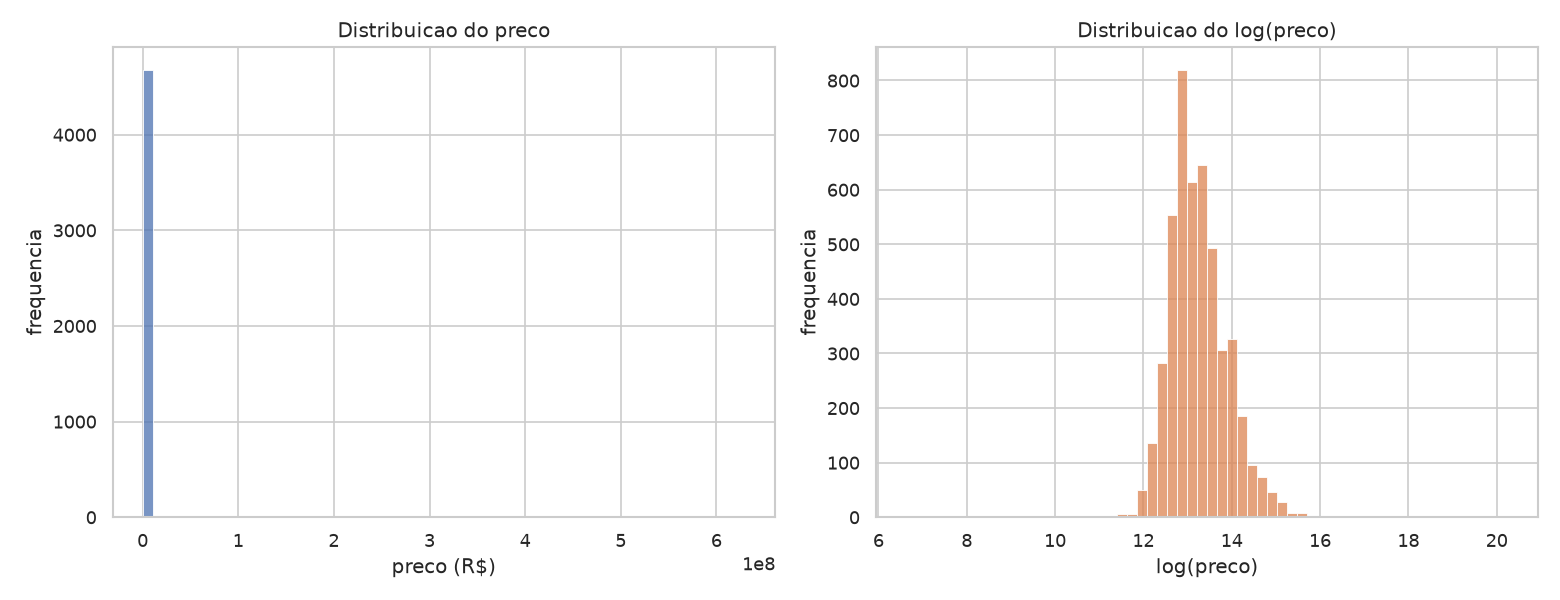
\includegraphics[width=1.0\textwidth]{eda_preco.png}
  \caption{Distribuição do preço bruto (esquerda) e de $\log(1+\text{preço})$ (direita).}
  \label{fig:preco}
\end{figure}

\subsection{Correlações e cardinalidade}

As correlações lineares das variáveis numéricas (\code{quartos}, \code{suites}, \code{vagas}, \code{area\_util}, \code{area\_extra}) com o preço bruto são todas muito fracas ($|r| < 0{,}05$, Figura~\ref{fig:corr}), o que reforça a necessidade da transformação logarítmica do \textit{target} e de \textit{features} de interação não-lineares (Seção~\ref{sec:features}).

\begin{figure}[H]
  \centering
  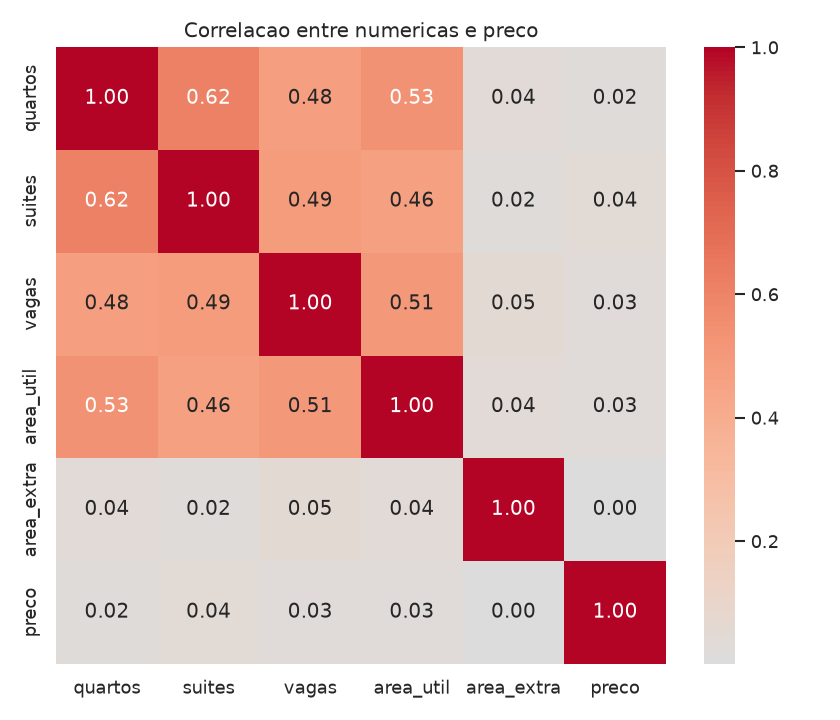
\includegraphics[width=0.7\textwidth]{eda_correlacoes.png}
  \caption{Matriz de correlação entre variáveis numéricas e o preço.}
  \label{fig:corr}
\end{figure}

O conjunto possui 4 tipos de imóvel (predominantemente ``Apartamento''), 66 bairros distintos no treino (alta cardinalidade, exigindo \textit{encoding} cuidadoso --- Seção~\ref{sec:encoding}) e 10 amenidades binárias (piscina, churrasqueira, sauna, vista para o mar, entre outras).

\section{Tratamento de \textit{Outliers}}
\label{sec:outliers}

Esta etapa teve o \textbf{maior impacto individual} de todo o trabalho. Os \textit{baselines} iniciais, treinados sem qualquer tratamento de \textit{outliers}, apresentaram RMSPE entre \textbf{196\% e 4867\%} --- um sinal inequívoco de que alguns poucos imóveis com preços absurdos estavam dominando a métrica percentual.

Aplicando o critério IQR $\times 3$ sobre $\log(1+\text{preço})$ no conjunto de treino, foram identificados 4 imóveis: dois de altíssimo valor (R\$~630 milhões e R\$~340 milhões, quase certamente erros de digitação), um de R\$~65 milhões, e um de apenas R\$~750 (provavelmente com dígitos faltando). A remoção desses 4 imóveis (de 4.683) derrubou o RMSPE do CatBoost de 2,083 para 0,238 --- uma redução de \textbf{88\%}, com reduções de até 92\% para o XGBoost (Tabela~\ref{tab:outliers}).

\begin{table}[H]
  \centering
  \caption{Impacto da remoção de \textit{outliers} (IQR $\times 3$) no RMSPE}
  \label{tab:outliers}
  \small\rowcolors{2}{rowalt}{white}
  \begin{tabular}{lcc}
    \toprule
    \rowcolor{headerblue}
    \color{white}\textbf{Modelo} & \color{white}\textbf{RMSPE com \textit{outliers}} & \color{white}\textbf{RMSPE sem \textit{outliers}} \\
    \midrule
    CatBoost~\cite{ref:catboost}  & 2,083 & 0,238 \\
    LightGBM~\cite{ref:lgbm}      & 2,594 & 0,249 \\
    XGBoost~\cite{ref:xgb}        & 3,369 & 0,268 \\
    \bottomrule
  \end{tabular}
\end{table}

Um corte adicional, mais agressivo, no percentil 99 do preço (removendo mais 47 imóveis do treino, que passou de 4.679 para \textbf{4.632} amostras) reduziu ainda mais o RMSPE, de 0,2306 para \textbf{0,2240}. Em nenhum momento o conjunto de teste foi alterado --- a remoção de \textit{outliers} ocorre exclusivamente no treino, para que o modelo não aprenda com dados espúrios.

\section{Transformação do \textit{Target}}
\label{sec:target}

Todo o treinamento foi conduzido sobre $y = \log(1+\text{preço})$, com as previsões convertidas de volta à escala original por $\hat{\text{preço}} = \exp(\hat{y}) - 1$. A justificativa é direta: como o RMSPE penaliza o erro \textbf{percentual}, e o erro percentual no espaço original é aproximadamente equivalente ao erro absoluto no espaço logarítmico, treinar em $\log(1+\text{preço})$ faz com que a função de perda usual dos modelos de \textit{gradient boosting} (baseada em erro absoluto/quadrático) já esteja, de forma aproximada, otimizando a métrica de avaliação real.

\section{Engenharia de \textit{Features}}
\label{sec:features}

Foram criadas diversas variáveis a partir dos atributos originais, guiadas pela análise exploratória e pelo conhecimento de domínio imobiliário (Tabela~\ref{tab:features}).

\begin{table}[H]
  \centering
  \caption{\textit{Features} criadas e motivação}
  \label{tab:features}
  \small\rowcolors{2}{rowalt}{white}
  \begin{tabular}{lp{9cm}}
    \toprule
    \rowcolor{headerblue}
    \color{white}\textbf{\textit{Feature}} & \color{white}\textbf{Motivação} \\
    \midrule
    \code{area\_total}            & Soma de \code{area\_util} e \code{area\_extra} --- área real disponível no imóvel. \\
    \code{log\_area\_util}        & Reduz assimetria da área, análogo à transformação do \textit{target}. \\
    \code{area\_por\_quarto}      & Área relativa ao número de cômodos --- captura ``amplidão'' independente do tamanho total. \\
    \code{total\_amenidades}      & Soma das 10 amenidades binárias --- proxy de padrão do imóvel. \\
    \code{categoria\_luxo}        & Flag: piscina + sauna + vista para o mar $\geq 2$ --- combinação típica de imóveis de alto padrão. \\
    \code{preco\_m2\_estimado}    & Mediana de (preço / \code{area\_util}) por bairro, com \textit{smoothing}, multiplicada pela área do imóvel --- dá ao modelo uma estimativa de preço já informada por localização \textbf{e} tamanho, em vez de deixá-lo aprender essa interação do zero. \\
    \code{quartos\_x\_area}, \code{vagas\_x\_area}, \code{luxo\_x\_area} & Interações entre quantidade (quartos, vagas, amenidades) e área --- capturam que o efeito de um cômodo extra difere conforme o tamanho do imóvel. \\
    \code{tipo\_x\_area}          & Interação entre cada categoria de \code{tipo} (\textit{one-hot}) e a área --- apartamentos e casas valorizam área de forma diferente. \\
    \bottomrule
  \end{tabular}
\end{table}

\section{Codificação de Variáveis Categóricas}
\label{sec:encoding}

\subsection{\textit{One-Hot Encoding}}

Aplicado a \code{tipo} (4 categorias: Apartamento, Casa, Loft, Quitinete).

\subsection{Bairro: \textit{Target Encoding} com \textit{smoothing} + \textit{frequency encoding}}

Com 66 categorias no treino, \code{bairro} exige uma codificação que capture o efeito de localização sem introduzir \textit{overfitting} excessivo. A abordagem final combina duas técnicas:

\begin{itemize}[leftmargin=2em, nosep]
  \item \textbf{\textit{Target encoding} com \textit{smoothing}} ($m=10$): $\text{TE}_b = \dfrac{n_b \cdot \bar{y}_b + m \cdot \bar{y}_{\text{global}}}{n_b + m}$, onde bairros com poucas amostras são puxados em direção à média global, seguindo a técnica descrita por Micci-Barreca~\cite{ref:micci}.
  \item \textbf{\textit{Frequency encoding}}: frequência relativa do bairro no treino, como \textit{feature} adicional.
\end{itemize}

\subsubsection{Abordagens testadas e descartadas}

\begin{itemize}[leftmargin=2em]
  \item \textbf{\textit{Target encoding} sem \textit{smoothing}} (mediana simples por bairro): RMSPE 0,2355, pior que a combinação \textit{smoothed} + \textit{frequency} (0,2320).
  \item \textbf{\textit{Frequency encoding} sozinho} (sem \textit{target encoding}): RMSPE 0,2405, o pior entre as variantes testadas.
  \item \textbf{\textit{Leave-One-Out} (LOO) \textit{encoding}}: para cada amostra, a média do bairro é calculada excluindo a própria amostra. RMSPE honesto de \textbf{0,3879} --- muito pior que o \textit{smoothing}, pois bairros com poucas amostras geram estimativas LOO extremamente ruidosas, sem a regularização que o \textit{smoothing} oferece.
  \item \textbf{\textit{Bug} de \textit{data leakage} detectado e corrigido}: a primeira implementação do LOO calculava as estatísticas por bairro \textbf{globalmente}, antes da validação cruzada, e só então aplicava a exclusão da própria amostra. Isso vazava informação entre \textit{folds} --- duas amostras do mesmo bairro em \textit{folds} de validação diferentes continuavam ``se enxergando'' pela estatística agregada compartilhada. O resultado era um RMSPE artificialmente baixo de \textbf{0,1627}, quase 30\% melhor que qualquer outra técnica testada em todo o trabalho --- grande demais para ser plausível. A correção recalculou o LOO separadamente dentro de cada \textit{fold}, usando somente o treino daquele \textit{fold}, revelando o verdadeiro desempenho (0,3879, muito pior). Esse episódio ilustra como o vazamento de dados em \textit{target encoding} pode produzir ganhos de validação cruzada enganosamente bons, como também discutido por Hastie et al.~\cite{ref:hastie}.
\end{itemize}

\textbf{Conclusão:} a combinação \textit{target encoding} com \textit{smoothing} + \textit{frequency encoding} foi mantida como codificação final do bairro.

\section{Modelagem}

Todos os modelos foram avaliados com \textbf{5-Fold Cross-Validation} sobre o RMSPE, já no conjunto de treino sem os 4 \textit{outliers} extremos (Seção~\ref{sec:outliers}). A Tabela~\ref{tab:baselines} apresenta os resultados com hiperparâmetros padrão.

\begin{table}[H]
  \centering
  \caption{RMSPE CV dos modelos base (após remoção de \textit{outliers})}
  \label{tab:baselines}
  \small\rowcolors{2}{rowalt}{white}
  \begin{tabular}{lcc}
    \toprule
    \rowcolor{headerblue}
    \color{white}\textbf{Modelo} & \color{white}\textbf{RMSPE CV} & \color{white}\textbf{Desvio} \\
    \midrule
    Regressão Linear                          & 3,8762 & 7,1787 \\
    Ridge                                     & 2,4124 & 4,2509 \\
    Lasso                                     & 31,6641 & 40,7961 \\
    Random Forest~\cite{ref:breiman}          & 0,2556 & 0,0135 \\
    Gradient Boosting                         & 0,2537 & 0,0178 \\
    LightGBM~\cite{ref:lgbm}                  & 0,2486 & 0,0093 \\
    XGBoost~\cite{ref:xgb}                    & 0,2683 & 0,0185 \\
    CatBoost~\cite{ref:catboost}              & \textbf{0,2380} & 0,0131 \\
    \bottomrule
  \end{tabular}
\end{table}

O CatBoost foi o melhor modelo individual (0,238), seguido de perto por LightGBM e XGBoost. Regressão Linear, Ridge e Lasso ficaram muito atrás --- esperado, dado que as correlações lineares com o preço são fracas (Figura~\ref{fig:corr}).

\section{Otimização de Hiperparâmetros}

A otimização foi conduzida com \textbf{Optuna}~\cite{ref:optuna} (busca bayesiana via TPE), com cada \textit{trial} avaliado por um \textit{split} 80/20 estratificado por quintis de $\log(1+\text{preço})$ --- garantindo que faixas de preço distintas (baratos, médios, caros) estivessem representadas tanto no treino quanto na validação de cada \textit{trial}.

\subsection{Impacto do número de \textit{trials}}

Foi conduzida uma primeira rodada com 50 \textit{trials} por modelo (RMSPE de validação: LightGBM 0,2144, XGBoost 0,2126, CatBoost 0,2102) e uma rodada estendida com 150/150/80 \textit{trials} para LightGBM/XGBoost/CatBoost respectivamente (RMSPE de validação: 0,2111, 0,2117, 0,2077). No Kaggle, a rodada estendida melhorou o score de \textbf{0,2469 para 0,2437}.

Esse resultado é \textbf{oposto} ao observado no Trabalho~1 (classificação de inadimplência), onde buscas mais longas de hiperparâmetros geraram \textit{overfitting} ao processo de validação e pioraram o desempenho no Kaggle. A explicação mais provável é o tamanho do conjunto de dados: o Trabalho~1 possuía 20.000 amostras, contra apenas 4.632 aqui --- em um espaço amostral menor, um orçamento maior de \textit{trials} tem mais espaço para explorar a região de hiperparâmetros sem necessariamente decorar particularidades de um único \textit{split}.

\begin{table}[H]
  \centering
  \caption{Hiperparâmetros finais (Optuna, 150/150/80 \textit{trials}, \textit{split} 80/20)}
  \label{tab:hyperparams}
  \small\rowcolors{2}{rowalt}{white}
  \begin{tabular}{lp{10.5cm}}
    \toprule
    \rowcolor{headerblue}
    \color{white}\textbf{Modelo} & \color{white}\textbf{Hiperparâmetros} \\
    \midrule
    LightGBM & \code{n\_estimators}=834, \code{max\_depth}=8, \code{num\_leaves}=51, \code{learning\_rate}=0,0059, \code{min\_child\_samples}=13, \code{subsample}=0,44, \code{colsample\_bytree}=0,46, \code{reg\_lambda}=0,52 \\
    XGBoost  & \code{n\_estimators}=1036, \code{max\_depth}=10, \code{learning\_rate}=0,0054, \code{min\_child\_weight}=19, \code{subsample}=0,66, \code{colsample\_bytree}=0,42, \code{reg\_alpha}=0,11, \code{reg\_lambda}=0,64 \\
    CatBoost & \code{iterations}=653, \code{depth}=10, \code{learning\_rate}=0,0165, \code{l2\_leaf\_reg}=1,17, \code{bagging\_temperature}=0,49, \code{random\_strength}=0,0064 \\
    \bottomrule
  \end{tabular}
\end{table}

\section{\textit{Ensemble}: Diagnóstico de Correlação}
\label{sec:ensemble}

Esta foi a etapa de maior ganho após o tratamento de \textit{outliers}. O \textit{blending} uniforme dos 3 \textit{boosters} otimizados não superava RMSPE de 0,2220 na validação cruzada, por melhor que fosse cada modelo individual. A causa foi investigada calculando a \textbf{matriz de correlação das previsões \textit{out-of-fold} (OOF)} de 8 modelos: os 3 \textit{boosters}, mais Random Forest~\cite{ref:breiman}, ExtraTrees, Ridge, ElasticNet e KNN.

\begin{table}[H]
  \centering
  \caption{Correlação das previsões OOF com o CatBoost}
  \label{tab:correlacao}
  \small\rowcolors{2}{rowalt}{white}
  \begin{tabular}{lc}
    \toprule
    \rowcolor{headerblue}
    \color{white}\textbf{Modelo} & \color{white}\textbf{Correlação com CatBoost (OOF)} \\
    \midrule
    XGBoost                & 0,995 \\
    LightGBM               & 0,995 \\
    Random Forest          & 0,992 \\
    ExtraTrees             & 0,992 \\
    Ridge                  & 0,967 \\
    ElasticNet             & 0,966 \\
    KNN                    & 0,962 \\
    \bottomrule
  \end{tabular}
\end{table}

O diagnóstico foi claro: LightGBM, XGBoost, CatBoost, Random Forest e ExtraTrees --- todos algoritmos baseados em árvores sobre as mesmas \textit{features} --- apresentam correlação $\geq 0{,}99$ entre si, errando quase sempre nos mesmos imóveis. Ridge, ElasticNet e KNN são estruturalmente diferentes (lineares e baseado em vizinhança) e, de fato, bem menos correlacionados ($\approx 0{,}96$) --- porém individualmente muito piores (RMSPE entre 0,267 e 0,276, contra $\approx 0{,}22$ dos \textit{boosters}).

Um \textit{blend} uniforme desses modelos fracos com os fortes pioraria o resultado. A solução foi \textbf{otimizar os pesos do \textit{blend}} via \code{scipy.optimize.minimize}~\cite{ref:scipy} (método SLSQP), com restrições $w_i \geq 0$ e $\sum_i w_i = 1$, minimizando diretamente o RMSPE das previsões OOF ponderadas:

\begin{table}[H]
  \centering
  \caption{Pesos otimizados do \textit{ensemble} final}
  \label{tab:pesos}
  \small\rowcolors{2}{rowalt}{white}
  \begin{tabular}{lc}
    \toprule
    \rowcolor{headerblue}
    \color{white}\textbf{Modelo} & \color{white}\textbf{Peso} \\
    \midrule
    CatBoost      & 0,39 \\
    LightGBM      & 0,32 \\
    XGBoost       & 0,14 \\
    KNN           & 0,13 \\
    Random Forest & 0,02 \\
    ElasticNet, Ridge, ExtraTrees & 0,00 \\
    \bottomrule
  \end{tabular}
\end{table}

O otimizador extraiu valor real do KNN --- individualmente o pior modelo do grupo --- justamente por seus erros serem menos correlacionados com os dos \textit{boosters}; um peso pequeno mas não-nulo (0,13) foi suficiente para reduzir o erro do \textit{ensemble} sem deixar o KNN dominar. ElasticNet, Ridge e ExtraTrees foram zerados pelo otimizador, indicando que não agregavam informação incremental relevante. O resultado foi RMSPE de \textbf{0,2205} na validação cruzada e \textbf{0,2393} no Kaggle --- o melhor score de todo o trabalho.

\section{Abordagens de \textit{Ensemble} Testadas e Descartadas}

\begin{itemize}[leftmargin=2em]
  \item \textbf{\textit{Stacking}} com meta-\textit{learner} Ridge sobre as previsões OOF dos 3 \textit{boosters}: RMSPE 0,2221, essencialmente empatado com o \textit{voting} uniforme (0,2220).
  \item \textbf{\textit{Blending} de submissões} já geradas (média em espaço logarítmico): não trouxe ganho --- as submissões tinham correlação $> 0{,}998$ entre si, um sintoma da mesma limitação diagnosticada na Seção~\ref{sec:ensemble}.
  \item \textbf{\textit{Feature selection}} (remoção de \textit{features} com importância $< 1\%$ no CatBoost): RMSPE 0,2242, pior que manter todas as \textit{features} (0,2234).
  \item \textbf{10 \textit{seeds} vs. 5 \textit{seeds}} no \textit{blend} multi-\textit{seed}: RMSPE idêntico (0,2223 em ambos) --- a redução de variância satura rapidamente, não compensando o custo computacional extra.
  \item \textbf{Regularização L2 dos pesos do \textit{ensemble}} ($\text{RMSPE} + \lambda \sum w_i^2$, $\lambda \in \{0; 0{,}001; 0{,}01; 0{,}1\}$): $\lambda = 0$ venceu; a penalização só piorou o resultado, sugerindo que a concentração de peso nos melhores modelos não era um artefato de \textit{overfitting} ao OOF.
  \item \textbf{\textit{Features} de palavras-chave} extraídas do campo de texto livre \code{diferenciais} (``gourmet'', ``mármore'', etc.): sem ganho algum, pois o campo na verdade usa um vocabulário fixo de combinações das 10 amenidades binárias, não texto livre genuíno.
  \item \textbf{Optuna direto no 5-fold CV} (em vez do \textit{split} 80/20) para o CatBoost: RMSPE 0,2237, contra 0,2235 do \textit{split} simples --- sem ganho, apesar do custo computacional 5 vezes maior por \textit{trial}.
  \item \textbf{Multi-\textit{seed} nos pesos otimizados} (\textit{pool} de 14 modelos: 3 \textit{boosters} $\times$ 3 \textit{seeds} + 5 modelos diversos): o RMSPE de validação cruzada melhorou para 0,2199, mas o Kaggle \textbf{piorou} para 0,2398 --- o otimizador concentrou quase todo o peso em \textit{seeds} específicas de cada \textit{booster}, um sinal de \textit{overfitting} ao conjunto OOF que não se confirmou no teste real, reforçando a importância de desconfiar de ganhos marginais de validação cruzada.
\end{itemize}

\section{Resultados}

A Tabela~\ref{tab:submissoes} resume a evolução das principais submissões ao Kaggle ao longo do trabalho.

\begin{table}[H]
  \centering
  \caption{Evolução das submissões ao Kaggle}
  \label{tab:submissoes}
  \small\rowcolors{2}{rowalt}{white}
  \begin{tabular}{p{8.5cm}c}
    \toprule
    \rowcolor{headerblue}
    \color{white}\textbf{Descrição} & \color{white}\textbf{RMSPE Kaggle} \\
    \midrule
    Baseline (\textit{blend}/\textit{voting} inicial)                     & 0,2535 \\
    + \textit{encoding} smoothed, \textit{features} de interação, corte de \textit{outliers} & 0,2479 \\
    + re-otimização Optuna no dataset limpo                                & 0,2469 \\
    + Optuna estendido (150/150/80 \textit{trials})                       & 0,2437 \\
    \textbf{+ \textit{ensemble} ponderado diverso (pesos otimizados)}     & \textbf{0,2393} \\
    \midrule
    (teste) multi-\textit{seed} nos pesos, 14 modelos                     & 0,2398 \\
    \bottomrule
  \end{tabular}
\end{table}

O melhor score obtido foi \textbf{0,2393}, uma melhoria de \textbf{5,6\%} em relação ao \textit{baseline} inicial (0,2535). A etapa de maior impacto isolado foi o tratamento de \textit{outliers} (Seção~\ref{sec:outliers}); a etapa de maior impacto \textit{fino} foi o diagnóstico de correlação do \textit{ensemble} (Seção~\ref{sec:ensemble}).

\section{Importância das \textit{Features}}

A Figura~\ref{fig:importance} apresenta a importância das 20 \textit{features} mais relevantes segundo o CatBoost otimizado. A Tabela~\ref{tab:importance} lista as 10 primeiras.

\begin{table}[H]
  \centering
  \caption{Top 10 \textit{features} por importância (CatBoost)}
  \label{tab:importance}
  \small\rowcolors{2}{rowalt}{white}
  \begin{tabular}{clc}
    \toprule
    \rowcolor{headerblue}
    \color{white}\textbf{\#} & \color{white}\textbf{\textit{Feature}} & \color{white}\textbf{Importância} \\
    \midrule
    1  & \code{vagas\_x\_area} (engenharia)              & 19,2\% \\
    2  & \code{log\_preco\_m2\_estimado} (engenharia)    & 8,8\% \\
    3  & \code{preco\_m2\_estimado} (engenharia)         & 8,4\% \\
    4  & \code{quartos\_x\_area} (engenharia)            & 7,6\% \\
    5  & \code{bairro\_target\_enc} (\textit{encoding})  & 6,3\% \\
    6  & \code{luxo\_x\_area} (engenharia)               & 6,3\% \\
    7  & \code{bairro\_preco\_m2} (engenharia)           & 5,7\% \\
    8  & \code{suites\_ratio\_quartos} (engenharia)      & 5,5\% \\
    9  & \code{bairro\_freq\_enc} (\textit{encoding})    & 5,4\% \\
    10 & \code{tipo\_Apartamento\_x\_area} (engenharia)  & 5,1\% \\
    \bottomrule
  \end{tabular}
\end{table}

Destaca-se que \textbf{todas} as 10 \textit{features} mais importantes foram criadas na etapa de engenharia de \textit{features} ou de \textit{encoding} (Seções~\ref{sec:features} e~\ref{sec:encoding}) --- nenhuma variável original bruta aparece no topo, validando fortemente o investimento nessas etapas. A variável \code{vagas\_x\_area} isoladamente concentra quase 20\% (19,2\%) da importância total, sugerindo que a interação entre vagas de garagem e área do imóvel é o sinal mais forte disponível para prever o preço. Chama atenção também que \textbf{três} das dez posições (\code{log\_preco\_m2\_estimado}, \code{preco\_m2\_estimado} e \code{bairro\_preco\_m2}) pertencem à família de \textit{features} de preço por m² descrita na Seção~\ref{sec:features} --- reforçando que essa estimativa informada por localização e tamanho é, de fato, um dos sinais mais úteis do modelo.

\begin{figure}[H]
  \centering
  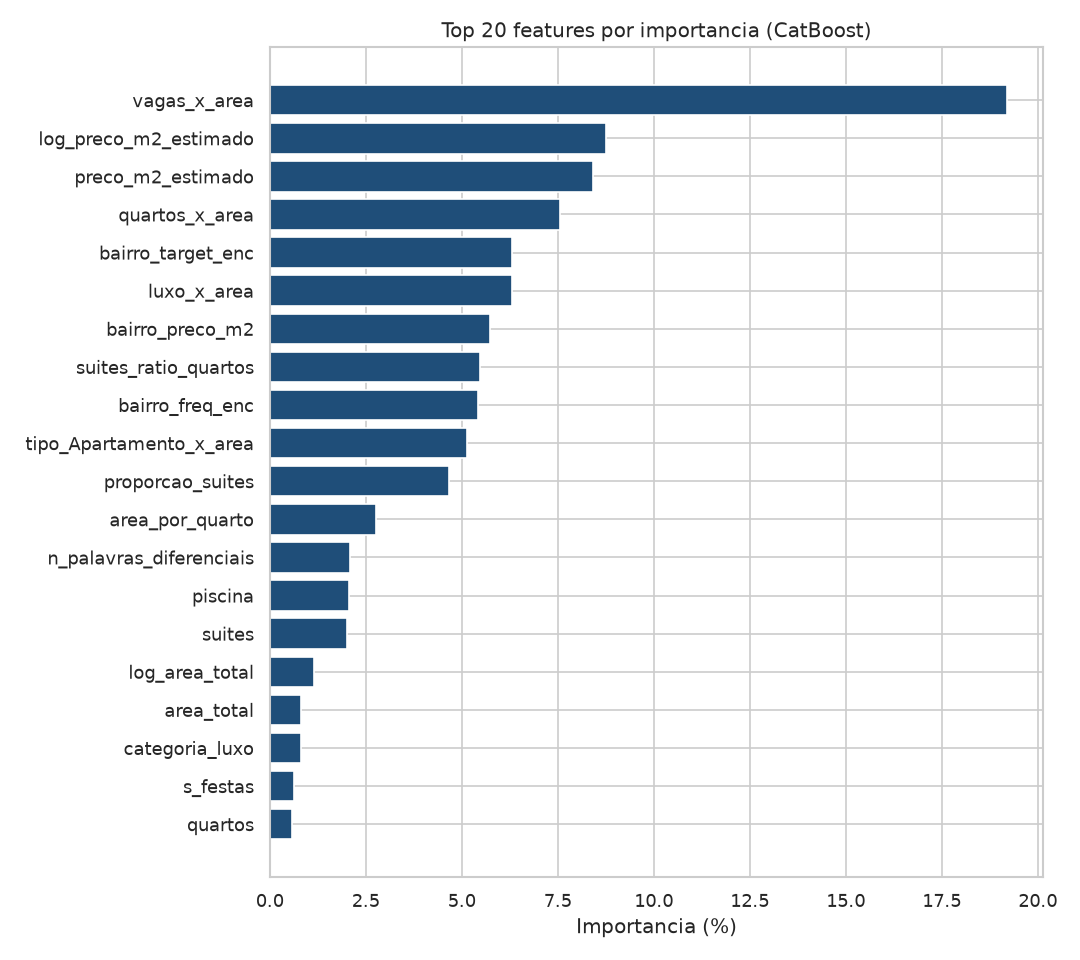
\includegraphics[width=1.0\textwidth]{feature_importance.png}
  \caption{Top 20 \textit{features} por importância no CatBoost otimizado.}
  \label{fig:importance}
\end{figure}

\section{Conclusões}

\begin{enumerate}[leftmargin=2em]
  \item \textbf{A transformação logarítmica do \textit{target}} é essencial quando a métrica de avaliação é percentual (RMSPE): treinar em $\log(1+\text{preço})$ aproxima a função de perda usual dos modelos da métrica real de avaliação.

  \item \textbf{O tratamento de \textit{outliers} teve o maior impacto individual} de todo o trabalho: remover apenas 4 de 4.683 amostras (0,09\% do treino) derrubou o RMSPE de aproximadamente 200\% para cerca de 24\%.

  \item \textbf{\textit{Target encoding} requer regularização (\textit{smoothing})}: a versão pura (\textit{Leave-One-Out}) mostrou-se ruidosa demais em categorias esparsas, e uma primeira implementação continha um \textit{bug} de vazamento de dados entre \textit{folds} que produzia ganhos de validação enganosamente otimistas --- um lembrete de que resultados bons demais merecem investigação antes de serem aceitos.

  \item \textbf{A correlação entre modelos limita o ganho de \textit{ensemble}}: 5 modelos baseados em árvores, por mais distintos que sejam em sua implementação (LightGBM, XGBoost, CatBoost, Random Forest, ExtraTrees), apresentaram correlação $\geq 0{,}99$ entre si e, portanto, pouco se complementaram.

  \item \textbf{Diversidade estrutural com pesos otimizados quebrou esse teto}: um modelo individualmente fraco (KNN, RMSPE 0,276) melhorou o \textit{ensemble} final porque seus erros ocorrem em lugares diferentes dos erros dos \textit{boosters} --- mas isso só funcionou porque os pesos foram otimizados (não uniformes), permitindo ao modelo fraco contribuir sem dominar.

  \item \textbf{Melhorias na validação cruzada nem sempre se traduzem no teste real}: a variante multi-\textit{seed} dos pesos otimizados melhorou o RMSPE de CV (0,2199) mas piorou no Kaggle (0,2398), evidenciando \textit{overfitting} ao conjunto \textit{out-of-fold} quando o espaço de otimização (14 modelos) é grande demais em relação aos dados disponíveis.

  \item \textbf{O número ótimo de \textit{trials} do Optuna depende do tamanho do conjunto de dados}: no Trabalho~1 (20.000 amostras), buscas mais longas pioraram a generalização; aqui (4.632 amostras), buscas mais longas melhoraram --- não existe uma regra universal, e a validação empírica em cada problema é indispensável.
\end{enumerate}

\newpage
\begin{thebibliography}{99}
\addcontentsline{toc}{section}{Referências}

\bibitem{ref:sklearn}
Pedregosa, F. et al. Scikit-learn: Machine Learning in Python. \textit{Journal of Machine Learning Research}, v.~12, p.~2825--2830, 2011.

\bibitem{ref:lgbm}
Ke, G. et al. LightGBM: A Highly Efficient Gradient Boosting Decision Tree. \textit{Advances in Neural Information Processing Systems (NeurIPS)}, v.~30, 2017.

\bibitem{ref:xgb}
Chen, T.; Guestrin, C. XGBoost: A Scalable Tree Boosting System. \textit{Proceedings of the 22nd ACM SIGKDD}, p.~785--794, 2016.

\bibitem{ref:catboost}
Prokhorenkova, L. et al. CatBoost: unbiased boosting with categorical features. \textit{Advances in Neural Information Processing Systems (NeurIPS)}, v.~31, 2018.

\bibitem{ref:optuna}
Akiba, T. et al. Optuna: A Next-generation Hyperparameter Optimization Framework. \textit{Proceedings of the 25th ACM SIGKDD}, p.~2623--2631, 2019.

\bibitem{ref:friedman}
Friedman, J. H. Greedy Function Approximation: A Gradient Boosting Machine. \textit{Annals of Statistics}, v.~29, n.~5, p.~1189--1232, 2001.

\bibitem{ref:breiman}
Breiman, L. Random Forests. \textit{Machine Learning}, v.~45, n.~1, p.~5--32, 2001.

\bibitem{ref:micci}
Micci-Barreca, D. A Preprocessing Scheme for High-Cardinality Categorical Attributes in Classification and Prediction Problems. \textit{ACM SIGKDD Explorations Newsletter}, v.~3, n.~1, p.~27--32, 2001.

\bibitem{ref:hastie}
Hastie, T.; Tibshirani, R.; Friedman, J. \textit{The Elements of Statistical Learning}. 2.~ed. New York: Springer, 2009.

\bibitem{ref:pandas}
McKinney, W. Data Structures for Statistical Computing in Python. \textit{Proceedings of the 9th Python in Science Conference}, p.~56--61, 2010.

\bibitem{ref:scipy}
Virtanen, P. et al. SciPy 1.0: Fundamental Algorithms for Scientific Computing in Python. \textit{Nature Methods}, v.~17, p.~261--272, 2020.

\end{thebibliography}

\end{document}
